
\documentclass[11pt]{article}
\usepackage[margin=1in]{geometry}
\usepackage{graphicx}
\usepackage{booktabs}
\usepackage{float}
\usepackage{hyperref}
\usepackage{amsmath}

\title{ADMET-AI vs SwissADME for Predicting Cardiac Drug Toxicity\\
\large Comparison on 25 Cardiac RODEO Drugs}
\author{Cardiac RODEO Project}
\date{\today}

\begin{document}
\maketitle

\begin{abstract}
This report compares two computational approaches for predicting drug-induced cardiotoxicity (DICT):
ADMET-AI (41 ADMET properties) and SwissADME (43 physicochemical properties).
We evaluate models trained on the DICTrank dataset (555 drugs) and models trained directly on 25 Cardiac RODEO drugs using Leave-One-Out Cross-Validation (LOOCV).
\end{abstract}

\section{Introduction}

Drug-induced cardiotoxicity (DICT) is a major concern in drug development. Two computational approaches are compared:

\begin{itemize}
    \item \textbf{ADMET-AI}: Uses 41 ADMET (Absorption, Distribution, Metabolism, Excretion, Toxicity) properties predicted from molecular structure
    \item \textbf{SwissADME}: Uses 43 physicochemical properties (MW, LogP, TPSA, etc.) computed from molecular structure
\end{itemize}

\section{Methods}

\subsection{Dataset}
The Cardiac RODEO dataset contains 25 drugs with experimentally determined cardiac outcomes:
\begin{itemize}
    \item Heart Damage: 20/25 positive
    \item Arrhythmia: 14/25 positive
    \item Concern (most): 15/25 positive
\end{itemize}

\subsection{DICTrank Models}
XGBoost models (500 trees, depth=12) were trained on the DICTrank dataset (555 drugs: 293 high DICT concern, 262 no concern) and applied to predict outcomes for the 25 Cardiac RODEO drugs.

\subsection{LOOCV Models}
New XGBoost models (100 trees, depth=3) were trained on the 25 Cardiac RODEO drugs using Leave-One-Out Cross-Validation to assess predictive performance with the actual cardiac outcomes as labels.

\section{Results}

\subsection{DICTrank-Trained Models}

These models were trained on clinical DICT concern labels, then evaluated on Cardiac RODEO experimental labels.

\begin{table}[H]
\centering
\caption{Performance of DICTrank-Trained Models on Cardiac RODEO Labels}
\begin{tabular}{llcc}
\toprule
\textbf{Model} & \textbf{Target} & \textbf{Accuracy} & \textbf{AUC} \\
\midrule
ADMET-AI & Heart Damage & 0.640 & 0.420 \\
SwissADME & Heart Damage & 0.600 & 0.600 \\
ADMET-AI & Arrhythmia & 0.640 & 0.662 \\
SwissADME & Arrhythmia & 0.680 & 0.571 \\
ADMET-AI & Concern (most) & 0.680 & 0.633 \\
SwissADME & Concern (most) & 0.640 & 0.713 \\

\bottomrule
\end{tabular}
\end{table}

\begin{figure}[H]
\centering
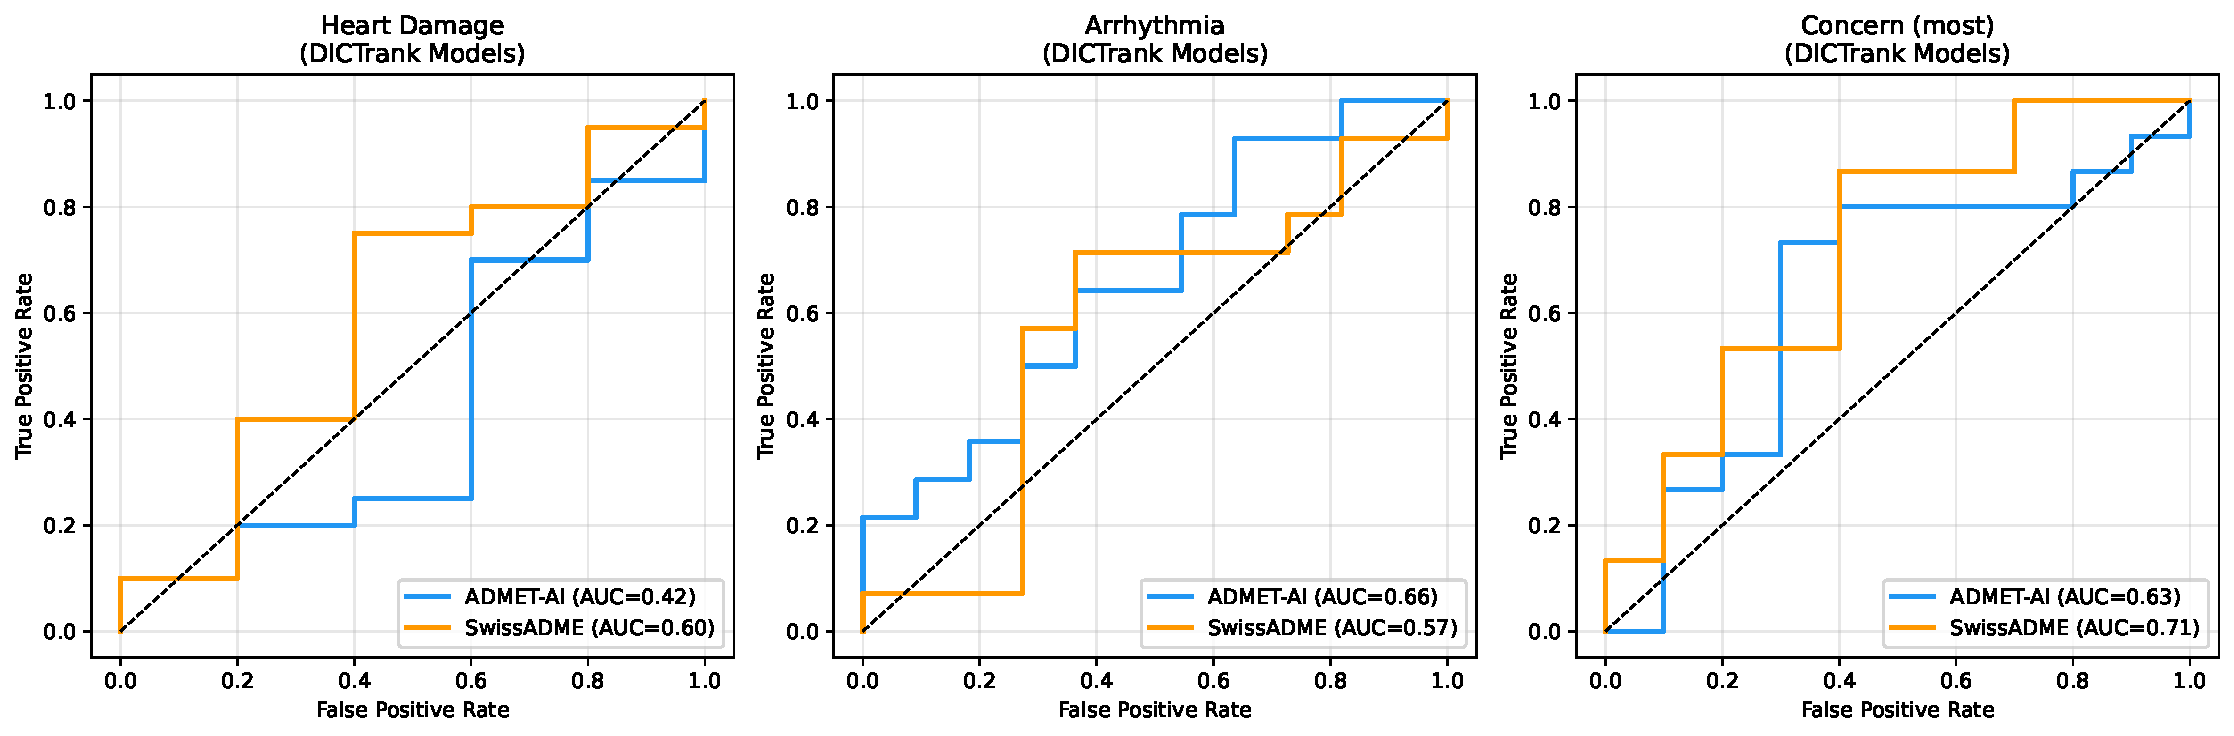
\includegraphics[width=\textwidth]{roc_dictrank_models.pdf}
\caption{ROC curves for DICTrank-trained models predicting Cardiac RODEO outcomes.}
\end{figure}

\subsection{LOOCV Models (Trained on 25 Drugs)}

These models were trained directly on the 25 Cardiac RODEO drugs using Leave-One-Out Cross-Validation.

\begin{table}[H]
\centering
\caption{Performance of LOOCV Models on Cardiac RODEO Drugs}
\begin{tabular}{llcc}
\toprule
\textbf{Model} & \textbf{Target} & \textbf{Accuracy} & \textbf{AUC} \\
\midrule
ADMET-AI & Heart Damage & 0.600 & 0.510 \\
SwissADME & Heart Damage & 0.720 & 0.530 \\
ADMET-AI & Arrhythmia & 0.600 & 0.630 \\
SwissADME & Arrhythmia & 0.400 & 0.344 \\
ADMET-AI & Concern (most) & 0.520 & 0.607 \\
SwissADME & Concern (most) & 0.720 & 0.553 \\

\bottomrule
\end{tabular}
\end{table}

\begin{figure}[H]
\centering
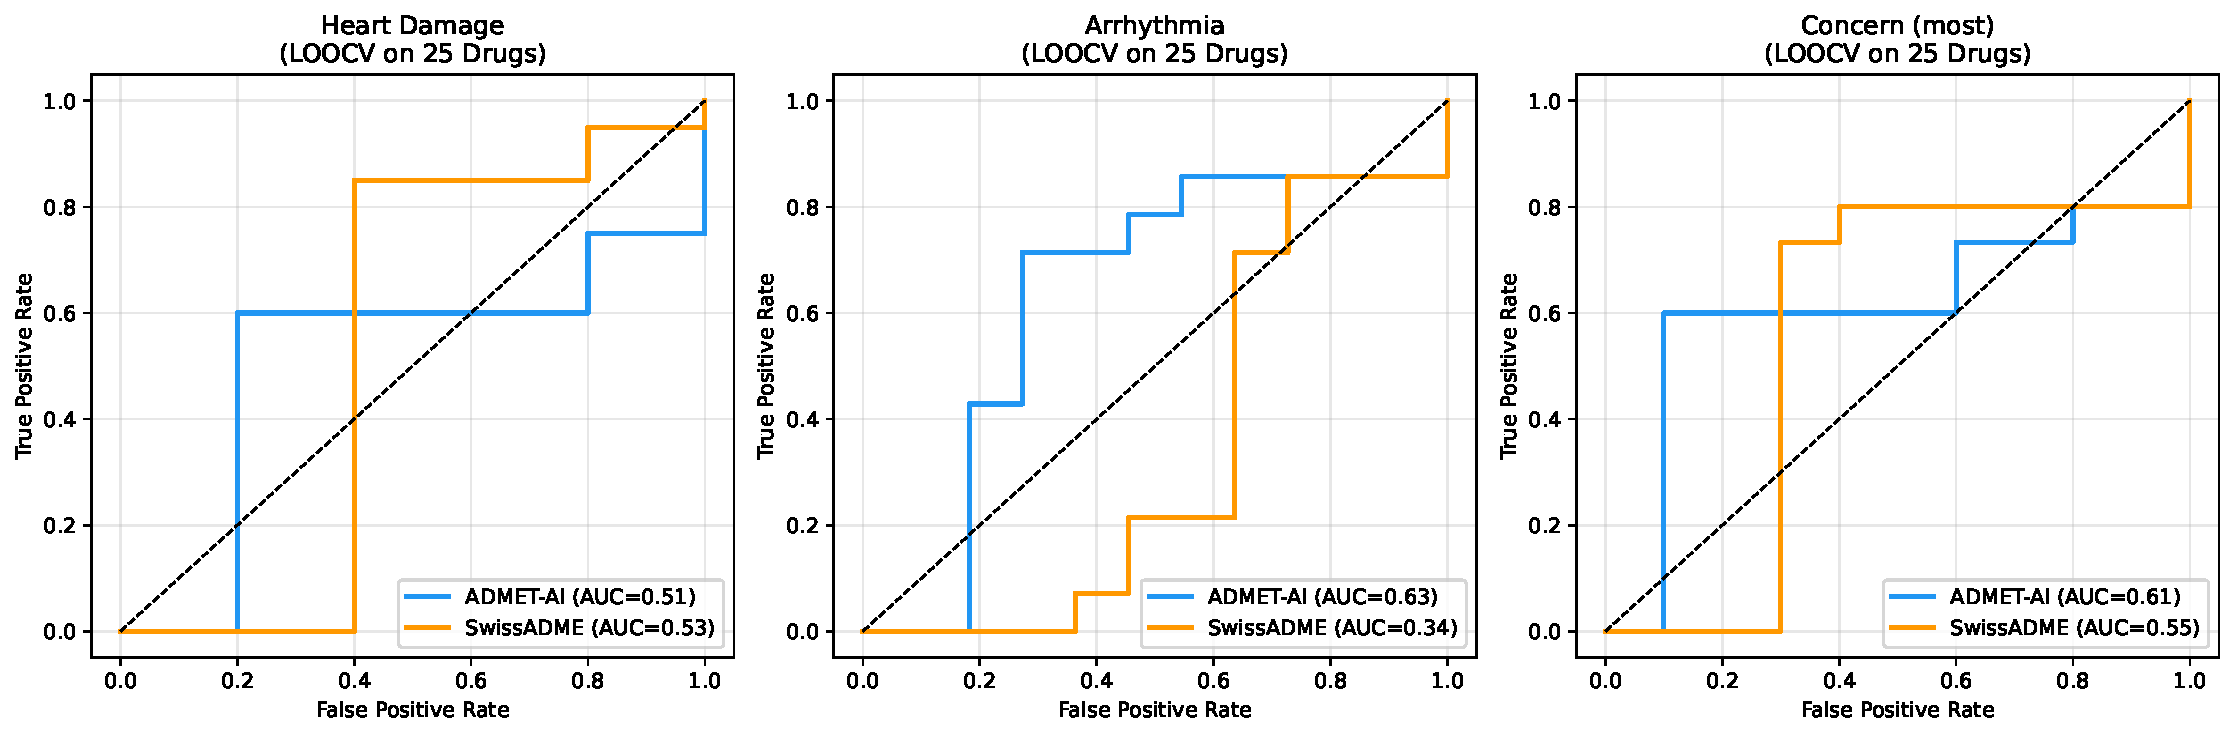
\includegraphics[width=\textwidth]{roc_loocv_models.pdf}
\caption{ROC curves for LOOCV models trained on 25 Cardiac RODEO drugs.}
\end{figure}

\subsection{Comparison Summary}

\begin{figure}[H]
\centering
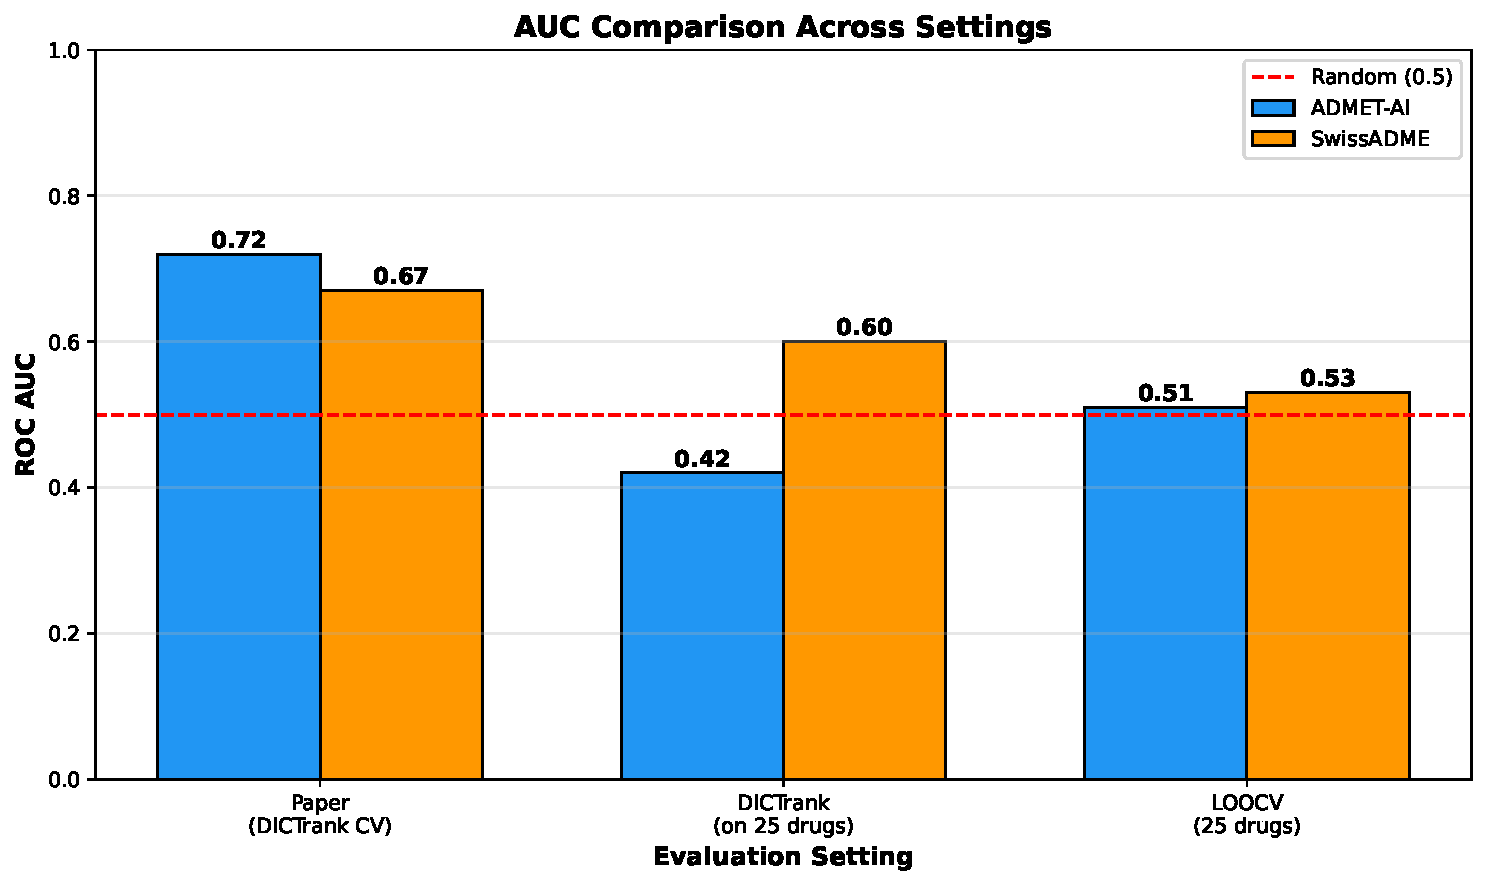
\includegraphics[width=\textwidth]{auc_comparison.pdf}
\caption{Comparison of AUC scores across all models and targets.}
\end{figure}

\section{Discussion}

Key observations:

\begin{enumerate}
    \item \textbf{DICTrank vs LOOCV}: Models trained on DICTrank (clinical DICT concern) do not perfectly predict Cardiac RODEO experimental outcomes, suggesting differences between clinical cardiotoxicity and organoid-measured cardiac effects.

    \item \textbf{ADMET-AI vs SwissADME}: The two feature sets capture different aspects of molecular properties, leading to different predictions for the same drugs.

    \item \textbf{Small Sample Size}: With only 25 drugs, LOOCV results should be interpreted cautiously due to high variance.
\end{enumerate}

\section{Conclusion}

This analysis demonstrates the utility and limitations of computational ADMET prediction for cardiac toxicity assessment. While models trained on large clinical datasets (DICTrank) provide useful risk estimates, validation on specific experimental systems requires careful interpretation.

\end{document}
